\documentclass[12pt,a4paper]{report}

\usepackage{styles/dolgozat}

\usepackage{listings}
\usepackage{styles/cpp}
\usepackage{styles/python}

\usepackage{tikz}
\usepackage{graphicx}

\usepackage{hyperref}

\begin{document}

\pagestyle{empty} %a címlapon ne legyen semmi=empty, azaz nincs fejléc és lábléc

% A Miskolci Egyetem címere
{\large
\begin{center}
\vglue 1truecm
\textbf{\huge\textsc{Szakdolgozat}}\\
\vglue 1truecm

\includegraphics[width=4.8truecm, height=4truecm]{images/me_logo.png}\\
\textbf{\textsc{Miskolci Egyetem}}
\end{center}}

\vglue 1.5truecm %függõleges helykihagyás

% A szakdolgozat címe, akár több sorban is
{\LARGE
\begin{center}
\textbf{A szakdolgozat címe}
\end{center}}

\vspace*{2.5truecm}
% A hallgató neve, évfolyam, szak(ok), a konzulens(ek) neve
{\large
\begin{center}
\begin{tabular}{c}
\textbf{Készítette:}\\
Csehi Máté\\
Programtervező informatikus
\end{tabular}
\end{center}
\begin{center}
\begin{tabular}{c}
\textbf{Témavezető:}\\
Piller Imre
\end{tabular}
\end{center}}
\vfill
% Keltezés: Hely, év
{\large
\begin{center}
\textbf{\textsc{Miskolc, 2021}}
\end{center}}

\newpage


\newpage

\pagestyle{empty}

%Feladatkiiras
\begin{flushleft}
\textsc{\bfseries Miskolci Egyetem}\\
Gépészmérnöki és Informatikai Kar\\
Alkalmazott Matematikai Intézeti Tanszék\hspace*{4cm}\hfil \textbf{Szám:}
\end{flushleft}
\vskip 0.5cm
\begin{center}
\large\textsc{\bfseries Szakdolgozat Feladat}
\end{center}
\vskip 0.5cm
Csehi Máté (GKDM8D) programtervező informatikus jelölt részére.\newline

\noindent\textbf{A szakdolgozat tárgyköre:} szimuláció, optimalizálás\newline

\noindent\textbf{A szakdolgozat címe:} Dobókockák alakjának meghatározása diszkrét eloszlásokhoz\newline

\noindent\textbf{A feladat részletezése:}

\medskip

\emph{Ide kell a feladatkiírásban szereplő szöveget betenni.}

\medskip

\emph{(Kisebb tagolás lehet benne, hogy jól nézzen ki.)}

\vfill

\noindent\textbf{Témavezető:} Piller Imre (egyetemi tanársegéd) \newline

% \noindent\textbf{Konzulens(ek):} (akkor kötelezõ, ha a témavezetõ nem valamelyik matematikai tanszékrõl való; de persze lehet egyébként is)\newline

\noindent\textbf{A feladat kiadásának ideje:} 2020. szeptember 23.\newline

%\noindent\textbf{A feladat beadásának határideje:}

\vskip 2cm

\hbox to \hsize{\hfil{\hbox to 6cm {\dotfill}\hbox to 1cm{}}}

\hbox to \hsize{\hfil\hbox to 3cm {szakfelelős}\hbox to 2cm{}}

\newpage

\vspace*{1cm}  
\begin{center}
\large\textsc{\bfseries Eredetiségi Nyilatkozat}
\end{center}
\vspace*{2cm}  

Alulírott \textbf{Csehi Máté}; Neptun-kód: \texttt{GKDM8D} a Miskolci Egyetem Gépészmérnöki és Informatikai Karának végzős Programtervező informatikus szakos hallgatója ezennel büntetőjogi és fegyelmi felelősségem tudatában nyilatkozom és aláírásommal igazolom, hogy \textit{Dobókockák alakjának meghatározása diszkrét eloszlásokhoz}
című szakdolgozatom saját, önálló munkám; az abban hivatkozott szakirodalom
felhasználása a forráskezelés szabályai szerint történt.\\

Tudomásul veszem, hogy szakdolgozat esetén plágiumnak számít:
\begin{itemize}
\item szószerinti idézet közlése idézőjel és hivatkozás megjelölése nélkül;
\item tartalmi idézet hivatkozás megjelölése nélkül;
\item más publikált gondolatainak saját gondolatként való feltüntetése.
\end{itemize}

Alulírott kijelentem, hogy a plágium fogalmát megismertem, és tudomásul veszem, hogy
plágium esetén szakdolgozatom visszautasításra kerül.

\vspace*{3cm}

\noindent Miskolc, \hbox to 2cm{\dotfill} .év \hbox to 2cm{\dotfill} .hó \hbox to 2cm{\dotfill} .nap

\vspace*{3cm}

\hspace*{8cm}\begin{tabular}{c}
\hbox to 6cm{\dotfill}\\
Hallgató
\end{tabular}



\newpage

\noindent 1.

\begin{tabular}{cl}
&szükséges (módosítás külön lapon) \\
A szakdolgozat feladat módosítása& \\
& nem szükséges\\
&\\
\hbox to 4cm{\dotfill}&\multicolumn{1}{c}{\hbox to 5cm{\dotfill}}\\
dátum& \multicolumn{1}{c}{témavezető(k)}
\end{tabular}
\vskip1.5mm

\noindent 2. A feladat kidolgozását ellenőriztem:

\vskip1.5mm

\begin{tabular}{l@{\hspace*{4cm}}l}
témavezető (dátum, aláírás):& konzulens (dátum, aláírás):\\
\dotfill&\dotfill\\
\dotfill&\dotfill\\
\dotfill&\dotfill
\end{tabular}

\vskip1.5mm

\noindent 3. A szakdolgozat beadható:

\vskip1.5mm

\begin{tabular}{@{\hspace*{1.3cm}}c@{\hspace*{2.1cm}}c}
\hbox to 4cm{\dotfill}&\multicolumn{1}{c}{\hbox to 5cm{\dotfill}}\\
dátum& \multicolumn{1}{c}{témavezető(k)}
\end{tabular}

\vskip1.5mm

\noindent 4.
\begin{tabular}[t]{@{}l@{\hspace*{1mm}}l@{\hspace*{1mm}}l@{}}
A szakdolgozat& \hbox to 3.5cm{\dotfill} &szövegoldalt\\
              & \hbox to 3.5cm{\dotfill} &program protokollt (listát, felhasználói leírást)\\
              &\hbox to 3.5cm{\dotfill}   &elektronikus adathordozót (részletezve)\\
              &\hbox to 3.5cm{\dotfill} & \\
              &\hbox to 3.5cm{\dotfill} &egyéb mellékletet (részletezve)\\
              &\hbox to 3.5cm{\dotfill} &\\
\end{tabular}
\newline tartalmaz.

\vskip1.5mm

\begin{tabular}{@{\hspace*{1.3cm}}c@{\hspace*{2.1cm}}c}
\hbox to 4cm{\dotfill}&\multicolumn{1}{c}{\hbox to 5cm{\dotfill}}\\
dátum& \multicolumn{1}{c}{témavezető(k)}
\end{tabular}

\noindent 5.

\begin{tabular}{ll}
&bocsátható\\
A szakdolgozat bírálatra& \\
& nem bocsátható\\
\end{tabular}

\vskip1.5mm

\noindent A bíráló neve: \hbox to 8cm{\dotfill}

\vskip4mm

\begin{tabular}{@{\hspace*{1.3cm}}c@{\hspace*{2.1cm}}c}
\hbox to 4cm{\dotfill}&\multicolumn{1}{c}{\hbox to 5cm{\dotfill}}\\
dátum& \multicolumn{1}{c}{szakfelelős}
\end{tabular}

\noindent 6.
\begin{tabular}[t]{@{}l@{\hspace*{1mm}}l@{\hspace*{1mm}}l@{}}
A szakdolgozat osztályzata& &\\
&a témavezető javaslata:& \hbox to 3cm{\dotfill}\\
&a bíráló javaslata:& \hbox to 3cm{\dotfill}\\
&a szakdolgozat végleges eredménye:& \hbox to 3cm{\dotfill}
\end{tabular}

\vspace*{4mm}

\noindent Miskolc, \hbox to 4.5cm{\dotfill} \hspace*{2.5cm}
\begin{tabular}[t]{cc}
\hbox to 6cm{\dotfill}\\
a Záróvizsga Bizottság Elnöke
\end{tabular}


\cleardoublepage
\pagenumbering{gobble}
\tableofcontents
\cleardoublepage
\pagenumbering{arabic}

\newpage

\pagestyle{fancy}

\Chapter{Bevezetés}

Dobókocka alatt alapvetően egy olyan, közel kocka alakú objektumra gondolhatunk, amelynek (tipikusan pöttyökkel) számozottak a lapjai. Az ezzel végzett dobássorozattól azt várjuk, hogy az $[1, 6]$ intervallumon lévő egész értékek egyenlő, $\dfrac{1}{6}$ valószínűséggel forduljanak elő.

A szakdolgozat témáját alapvetően két ötlet motiválja. Egyrészt a dobáshoz használt testnek nem szükségszerű kocka alakúnak lennie, más konvex testek is alkalmasak lehetnek arra, hogy egy adott diszkrét eloszlás szerint véletlenszerű értékeket szolgáltassanak. Másrészt, a testhez az eloszlás meghatározásának az inverz problémája is megoldható bizonyos esetekben.
A szakdolgozat ezen problémát igyekszik körüljárni, és heurisztikus módszerekkel egy adott, diszkrét eloszlás alapján becslést adni egy olyan testre, amely lapjaihoz a megfelelő valószínűségek tartoznak.

A vizsgálatokhoz szükség lesz egy keretrendszerre. Ennek elkészítését részletesen bemutatja a dolgozat. Ennek az egyik lényeges eleme egy olyan fizikai szimulátor, amely egy testet le tud ejteni, és meg tudja azt vizsgálni, hogy bizonyos idő elteltével melyik lapján áll meg.

% Ehhez a problémakörhöz kell egy fizikai szimulációs környezetet létrehozni, ami a dobási kísérletek elvégzéséért felel, valamint a testeknek egy általános reprezentációja, amiken a módosításokat könnyen el tudjuk végezni.

Részletezésre kerül majd, hogy egy dobássorozat alapján hogyan lehet azt megállapítani, hogy az elvárt és a kapott eloszlások megegyeznek-e. Az ehhez szükséges hibametrikák bemutatását követően olyan algoritmusokról lesz szó, amelyek a test csúcspontjainak elmozdításával keresik a problématérben az optimális testet.

A probléma megoldása nem triviális, egy érdekes optimalizálási feladat.
A módosításoknál figyelnünk kell az előfordulási arányok mellett a test konvexitására, és a nem háromszög alakú oldallapok síkban maradására, hogy ne "törjön" több háromszög alakú oldalra.

%Az optimalizálások során azt feltételezzük, hogy a keresett test létezik, de pontos egyezés helyett valamilyen hiba szerint fogjuk az alakzatokat elfogadni.
%A dolgozatban több különböző hibaszámítást fogunk megvizsgálni, és ezeket fogjuk összehasonlítani, hogy számunkra melyik használata lenne a legelőnyösebb.

A dolgozat a problémát teljes általánosságában nem oldja meg. Egy adott diszkrét eloszláshoz tartozó valószínűségi változó felvehető értékeinek száma alapján közvetlenül adottnak tekintjük a test topológiáját. Általánosságban külön vizsgálatot igényelne, hogy létezhet-e egyáltalán az adott eloszláshoz megfelelő test. A megoldhatósági probléma egzakt felírása helyett azt remélhetjük, hogy az optimalizáláshoz használt heurisztika az egyes iterációkhoz tartozó hibákkal jelzi majd, hogy milyen pontossággal sikerült közelíteni az elvárt eloszlást.

% A szakdolgozatom célja egy olyan program megírása, amely egy adott testet úgy módosít, hogy a testet dobókockaként használva az oldalak előfordulása az általunk megadott értékekhez közelítenek.
%Azért nem bízzuk a test teljes generálását a programra, mert az egyes $n$-oldalú testekhez nem egy testháló létezik, és így több testhálóhoz is le tudjuk tesztelni a programot.

A dolgozatban a vizsgálatokhoz elkészített szoftver felépítése és működése is kifejtésre kerül. Láthatunk példákat, amelyekben a konvergencia és a becsléssel kapott test is szemléltetésre kerül.

% A dolgozatban részletes leírásra kerül a szimuláció felépítése, az adatok tárolása és az eloszlások közötti távolság mérése.
\Chapter{Koncepció}

\Section{A fejezet célja}

Ez a fejezet még nem a saját eredményekkel foglalkozik, hanem bemutatja, mi a problémakör, milyen módszerekkel, milyeneredményeket sikerült elérni eddig másoknak.

A hivatkozások jelentős része ehhez a fejezethez szokott kötődni.
(Egy hivatkozás például így néz ki \cite{coombs1987markup}.)
Itt lehet bemutatni a hasonló alkalmazásokat.

\Section{Tartalom és felépítés}

A fejezet tartalma témától függően változhat. Az alábbiakat attól függően különböző arányban tartalmazhatják.
\begin{itemize}
\item Irodalomkutatás. Amennyiben a dolgozat egy módszer kidolgozására, kifejlesztésére irányul, akkor itt lehet részletesen végignézni (módszertani vagy időrendi bontásban), hogy az eddigiekben milyen eredmények születtek a témakörben.
\item Technológia. Mivel jellemzően kutatásról vagy szoftverfejlesztésről van szó, ezért annak a jellemző elemeit, technikai részleteit itt kell bemutatni.
Ez tehát egy módszeres bevezetés ahhoz, hogy ha valaki nem jártas a témakörben, akkor tudja, hogy a dolgozat milyen aktuálisan elérhető eredményeket, eszközöket használt fel.
\item Piackutatás. Bizonyos témáknál új termék vagy szolgáltatás kifejlesztése a cél.
Ekkor érdemes annak alaposan utánanézni, hogy aktuálisan milyen eszközök érhetők el a piacon.
Ez szoftverek esetében a hasonló alkalmazások bemutatását, táblázatos formában történő összehasonlítását jelentheti.
Szerepelhetnek képek és észrevételek a viszonyításként bemutatott alkalmazásokhoz.
\item Követelmény specifikáció. Külön szakaszban érdemes részletesen kitérni az elkészítendő alkalmazással kapcsolatos követelményekre.
Ehhez tartozhatnak forgatókönyvek (\textit{scenario}-k).
A szemléletesség kedvéért lehet hozzájuk képernyőkép vázlatokat is készíteni, vagy a használati eseteket más módon szemléltetni.
\end{itemize}

\Section{Amit csak említés szintjén érdemes szerepeltetni}

Az olvasóról annyit feltételezhetünk, hogy programozásban valamilyen szinten járatos, és a matematikai alapfogalmakkal sem ebben a dolgozatban kell megismertetni.
A speciális eszközök, programozási nyelvek, matematikai módszerekk és jelölések persze jó, hogy ha említésre kerülnek, de nem kell nagyon belemenni a közismertnek tekinthető dolgokba.

\Chapter{Szimulációs környezet}

\Section{A test reprezentációja}

A szimuláció során a test csak a $z=0$ síkkal fog érintkezni, és arról fog visszapattanni, így nem kell az olyan esetekkel foglalkoznunk, hogy az oldallapján, vagy egy élén fog valamivel érintkezni.
Ha véletlenül mégis egyszerre érintkezne a test éle vagy oldallapja a $z=0$ síkkal, akkor elegendő az élhez vagy oldallaphoz tartozó csúcspontokra elvégezni egyszerre a visszapattanást.
Emiatt csak a csúcspontokat, valamint az oldallapokon lévő csúcspontok indexét fogjuk eltárolni.

Az egyszerűbb számítások miatt nem szilárd objektumként kezeljük a testet, 	hanem egy pontokból és rugókból álló halmaznak.
Minden csúcspont közé, egy rugót feszítünk ki, amely a hozzá tartozó végpontokat igyekszik az eredeti távolságukban tartani.
Emiatt a testnek zselatinos jellege lesz, és ennek mértéke a rugóállandóval befolyásolható.

A dolgozat során csak a konvex testekkel fogunk foglalkozni, mivel könnyen belátható, hogy konkáv testek esetében lenne olyan oldallap, amelyre nem tud érkezni a dobás során a test.
Emiatt a módosítások után egy konvexitás vizsgálatot kell elvégeznünk a testen.
Ha a test konvex, akkor bármely oldallapjára nézve a pontok, amelyek nem csúcspontjai az oldalnak, ugyan abban az oldallap síkja által határolt félsíkban helyezkednek el.
Ehhez a vizsgálathoz fel kell írnunk minden oldallap síkjának az egyenletét, és a lapon kívüli pontokat vissza kell helyettesítenünk.
Ha minden pont ugyanabban a félsíkban található, akkor a behelyettesítéssel kapott értékek előjele meg fog egyezni.

Az oldallapok síkját úgy számoljuk, hogy az első három csúcspontjára ($P_1(x_1, y_1, z_1)$, $P_2(x_2, y_2, z_2)$ és $P_3(x_3, y_3, z_3)$) illesztjük a síkot az alábbi egyenletet használva:

\[
det(A)=0,\quad \text{ahol } A = 
\begin{bmatrix}
	x & y & z & 1 \\
	x_1 & y_1 & z_1 & 1 \\
	x_2 & y_2 & z_2 & 1 \\
	x_3 & y_3 & z_3 & 1
\end{bmatrix}
\]
\newpage

\begin{proof}
A $P_1(x_1, y_1, z_1)$, $P_2(x_2, y_2, z_2)$ és $P_3(x_3, y_3, z_3)$ pont által meghatározott sík normálvektorja:
\[
\begin{array}{c}
	\vec{n}=\overrightarrow{P_1 P_2}\times\overrightarrow{P_1 P_3}=(x_2-x_1, y_2-y_1, z_2-z_1)\times(x_3-x_1, y_3-y_1, z_3-z_1)=\\
	=
	\begin{vmatrix}
		\vec{i} & \vec{j} & \vec{k} \\
		x_2-x_1 & y_2-y_1 & z_2-z_1 \\
		x_3-x_1 & y_3-y_1 & z_3-z_1
	\end{vmatrix}=\\
	= ((y_2-y_1)(z_3-z_1)-(z_2-z_1)(y_3-y_1))\vec{i}+\\
	+ ((z_2-z_1)(x_3-x_1)-(x_2-x_1)(z_3-z_1))\vec{j}+\\
	+ ((x_2-x_1)(y_3-y_1)-(y_2-y_1)(x_3-x_1))\vec{k}
\end{array}
\]
A normálvektor és a $P1$ által felírt sík egyenlete:
\[
\begin{array}{c}
	A(x-x_1)+B(y-y_1)+C(z-z_1)=\\
	=((y_2-y_1)(z_3-z_1)-(z_2-z_1)(y_3-y_1))(x-x_1)+\\
	+((z_2-z_1)(x_3-x_1)-(x_2-x_1)(z_3-z_1))(y-y_1)+\\
	+((x_2-x_1)(y_3-y_1)-(y_2-y_1)(x_3-x_1))(z-z_1)=\\
	=(y_2 z_3 - y_1 z_3 - y_2 z_1 + y_1 z_1 - y_3 z_2 + y_3 z_1 + y_1 z_2 - y_1 z_1)(x-x_1)+\\
	+(x_3 z_2 - x_3 z_1 - x_1 z_2 + x_1 z_1 - x_2 z_3 + x_1 z_3 + x_2 z_1 - x_1 z_1)(y-y_1)+\\
	+(x_2 y_3 - x_1 y_3 - x_2 y_1 + x_1 y_1 - x_3 y_2 + x_3 y_1 + x_1 y_2 - x_1 y_1)(z-z_1)=\\
	=(y_2 z_3 - y_1 z_3 - y_2 z_1 - y_3 z_2 + y_3 z_1 + y_1 z_2)(x-x_1)+\\
	+(x_3 z_2 - x_3 z_1 - x_1 z_2 - x_2 z_3 + x_1 z_3 + x_2 z_1)(y-y_1)+\\
	+(x_2 y_3 - x_1 y_3 - x_2 y_1 - x_3 y_2 + x_3 y_1 + x_1 y_2)(z-z_1)=\\
	=(y_2 z_3 - y_1 z_3 - y_2 z_1 - y_3 z_2 + y_3 z_1 + y_1 z_2)x+\\
	+(x_3 z_2 - x_3 z_1 - x_1 z_2 - x_2 z_3 + x_1 z_3 + x_2 z_1)y+\\
	+(x_2 y_3 - x_1 y_3 - x_2 y_1 - x_3 y_2 + x_3 y_1 + x_1 y_2)z-\\
	- x_1 y_2 z_3 + x_1 y_1 z_3 + x_1 y_2 z_1 + x_1 y_3 z_2 - x_1 y_3 z_1 - x_1 y_1 z_2 -\\
	- x_3 y_1 z_2 + x_3 y_1 z_1 + x_1 y_1 z_2 + x_2 y_1 z_3 - x_1 y_1 z_3 - x_2 y_1 z_1 -\\
	- x_2 y_3 z_1 + x_1 y_3 z_1 + x_2 y_1 z_1 + x_3 y_2 z_1 - x_3 y_1 z_1 - x_1 y_2 z_1 =\\
	=(y_2 z_3 - y_1 z_3 - y_2 z_1 - y_3 z_2 + y_3 z_1 + y_1 z_2)x+\\
	+(x_3 z_2 - x_3 z_1 - x_1 z_2 - x_2 z_3 + x_1 z_3 + x_2 z_1)y+\\
	+(x_2 y_3 - x_1 y_3 - x_2 y_1 - x_3 y_2 + x_3 y_1 + x_1 y_2)z-\\
	- x_1 y_2 z_3 - x_2 y_3 z_1 - x_3 y_1 z_2 + x_3 y_2 z_1 + x_2 y_1 z_3  + x_1 y_3 z_2 = 0
\end{array}
\]
A $P_1(x_1, y_1, z_1)$, $P_2(x_2, y_2, z_2)$ és $P_3(x_3, y_3, z_3)$ pont által meghatározott sík egyenlete a feltételezésünk szerint:
\[
\begin{array}{c}
	A =
	\begin{vmatrix}
		x & y & z & 1 \\
		x_1 & y_1 & z_1 & 1 \\
		x_2 & y_2 & z_2 & 1 \\
		x_3 & y_3 & z_3 & 1
	\end{vmatrix}
	 = x
	\begin{vmatrix}
	 	y_1 & z_1 & 1 \\
	 	y_2 & z_2 & 1 \\
	 	y_3 & z_3 & 1
	\end{vmatrix}
	- y
	\begin{vmatrix}
		x_1 & z_1 & 1 \\
		x_2 & z_2 & 1 \\
		x_3 & z_3 & 1
	\end{vmatrix}
	+ z
	\begin{vmatrix}
		x_1 & y_1 & 1 \\
		x_2 & y_2 & 1 \\
		x_3 & y_3 & 1
	\end{vmatrix}
	-
	\begin{vmatrix}
		x_1 & y_1 & z_1 \\
		x_2 & y_2 & z_2 \\
		x_3 & y_3 & z_3
	\end{vmatrix}
	=\\
	=(y_2 z_3 - y_1 z_3 - y_2 z_1 - y_3 z_2 + y_3 z_1 + y_1 z_2)x+\\
	+(x_3 z_2 - x_3 z_1 - x_1 z_2 - x_2 z_3 + x_1 z_3 + x_2 z_1)y+\\
	+(x_2 y_3 - x_1 y_3 - x_2 y_1 - x_3 y_2 + x_3 y_1 + x_1 y_2)z-\\
	- x_1 y_2 z_3 - x_2 y_3 z_1 - x_3 y_1 z_2 + x_3 y_2 z_1 + x_2 y_1 z_3  + x_1 y_3 z_2 = 0
\end{array}
\]
Mivel ugyan azt az egyenletet kaptuk, így beláthatjuk hogy a sík egyenlete megegyezik a $det(A)=0$ egyenlettel.
\end{proof}

Az egyenlet ilyen felírása azért előnyös a számunkra, mert a \texttt{numpy} könyvtár tartalmaz függvényt, amely mátrix determinánst számol.
Így csak a mátrix felírását kell megoldanunk, az első sorába behelyettesíteni a vizsgált pont koordinátáit majd a mátrix determinánsának előjele alapján eldönteni, hogy melyik félsíkon található a pont.
Nem szükséges tudnunk, hogy a pontok pontosan melyik félsíkban helyezkednek el, minket csak az érdekel, hogy oldalakra nézve minden vizsgált pontra a $det(A)$ érték előjele azonos legyen.
Ennek a megvalósításához az értékekhez rendelt \texttt{np.linalg.det(A) < 0} logikai értéket fogjuk eltárolni egy halmazban, majd a halmaz méretéről meg tudjuk állapítani, hogy összesen mennyi féltérben helyezkednek el a vizsgált pontok.
Ha minden oldal esetén a halmazban lévő elemek száma 1, akkor a test konvex.
\begin{python}
def getPlaneOfFace(self, face):
    f = list(face)
    A = np.matrix([self.particles[f[0]].position,
                   self.particles[f[1]].position,
                   self.particles[f[2]].position])

    p = np.array([0, 0, 0])
    one = np.array([[1], [1], [1], [1]])

    A = np.vstack([p, A])
    A = np.append(A, one, axis=1)

    return A

def isConvex(self):
    for face in self.faces:
        A = self.getPlaneOfFace(face)
        sign = set()

        for i in range(self.n):
            if i not in face:
                A[0, :3] = self.particles[i].position
                sign.add(np.linalg.det(A) < 0)

        if len(sign)!=1:
            return False

    return True
\end{python}

A fent említett metódusok a \texttt{Dice} osztályhoz tartoznak, amely egyszerre felel a test reprezentálásáért, a fizikai szimulációk elvégzéséért valamint a test későbbi módosításáért is.
Az osztály attribútumaiban tároljuk a testet leíró paramétereket: egy-egy listát a csúcspontokról és a közöttük kifeszített rugókról, a csúcsok számát, valamint egy listát az oldallapokat határoló pontok halmazaiból.
Magát a \texttt{Dice} osztályt nem lehet példányosítani, mert a pontok inicializálására szolgáló metódus nincs implementálva, így csak az ebből származtatott osztályokból tudunk példányt készíteni.
\begin{python}
class Dice:
    def __init__(self):
        self.n
        self.partciles = []
        self.springs = []
        self.faces = []
        self.initVerticies()
        self.initSprings()

    def initVerticies(self):
        raise NotImplementedError

    def initSprings(self):
        for i in range(self.n - 1):
            for j in range(i + 1, self.n):
                	self.springs.append(Spring(self.particles[i],
                	                           self.particles[j]))
\end{python}
Minden testhez egy külön kell létrehoznunk egy gyerekosztályt, amely \texttt{initVerticies} metódusában beállítjuk a pontokat, oldalakat, csúcsok számát a kívánt testünkhöz.
A program teszteléséhez az alábbi négy testet fogjunk vizsgálni illetve módosítani: tetraéder, dupla tetraéder, kocka és oktaéder.
\begin{remark}
A dupla tetraéder alatt egy olyan hatoldalú testet értünk, amelyet két tetraéder összeragasztásával kapunk.
\end{remark}

\begin{figure}[h!]
	\centering
	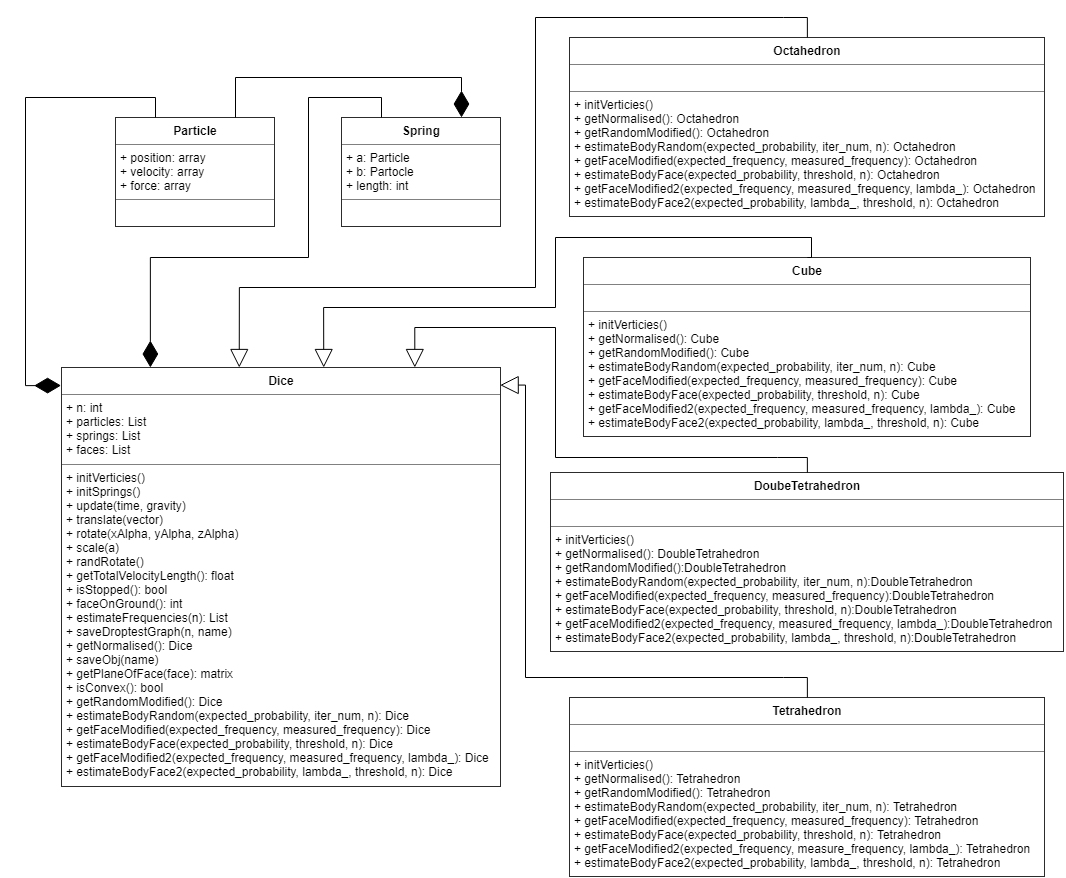
\includegraphics[width=\textwidth]{images/uml.png}
	\caption{Osztály diagram.}
	\label{fig:uml}
\end{figure}

\SubSection{Pontok}

A pontok felelnek a test mozgásáért, minden fizikai információt itt tárolunk el.
A szimulálás során a rá ható erőket, a mozgásvektorát, valamint a pozícióját tároljuk el.
Minden csúcs súlyát egységnyinek tekintjük, ezért nem foglalkozunk vele.
\begin{python}
class Particle:
    def __init__(self, a = [0, 0, 0]):
        self.position = np.array(a, dtype=float) 
        self.velocity = np.array([0, 0, 0], dtype=float)
        self.force = np.array([0, 0, 0], dtype=float)

    def __str__(self):
        return "({:.3f}, {:.3f}, {:.3f})".format(*self.position)
\end{python}

\SubSection{Rugók}

A rúgók felelnek a pontok helyén tartásáért.
Minden rúgó rugóállandóját ugyan akkorának tekintjük, ezzel szemléltetve, hogy homogén testet vizsgálunk.
Ezen okból nem tároljuk ez a rugóállandót, hanem konstans értékkel számolunk.

A test módosítása után a rugókat újra kell inicializálni, hogy a pontok közötti új távolságot próbálja meg folyamatosan tartani.
Ha ezt nem tennénk meg, a dobás szimulálása után a test visszaugrana a módosítás előtti állapotába.
\begin{python}
class Spring:
    def __init__(self, a, b):
        self.a = a
        self.b = b
        self.length = np.linalg.norm(self.b.position - self.a.position)
	
    def __str__(self):
        return f"{self.a}; {self.b}; {self.length}"
\end{python}

\SubSection{Exportálás fájlba}

A programunk nem rendelkezik háromdimenziós megjelenítővel, ezért a testek megjelenítését külső programmal kell megtennünk, amihez a testeket \texttt{obj} formátumú fájlba mentjük ki.
Azért erre esett a választás, mert ezeket a fájlokat a legtöbb 3D szerkesztő meg tudja nyitni, valamint az adattárolása megegyezik az általunk használt tárolási móddal.

\begin{python}
def saveObj(self, name):
    filepath= f"objects/{name}.obj"

    with open(filepath, 'w') as f:
        f.write("# OBJ file\n")
        for particle in self.particles:
            f.write("v {} {} {}\n".format(*particle.position))
        for i in range(len(self.faces)):
            f.write("f")
            for p in self.faces[i]:
                f.write(f" {p + 1}")
            f.write("\n")

    print(f"Obj file saved to '{filepath}'.")
\end{python}

\Section{Dobások}

A kockadobások szimulálását úgy végezzük, hogy a testet egy adott magasságig felemeljük, majd onnan ejtjük le a $z=0$ síkra.
A fizikai számításokat a \texttt{Dice.update} metódus végzi el az alábbi lépéssorozatot követve:
\begin{enumerate}
	\item A csúcspontokra ható erőt beállítja a gravitációra
	\item Az erőhöz hozzáadja a mozgásvektorját
	\item Kiszámítja a rugóerőket, és rendre hozzáadja/kivonja az erőkből
	\item Ha egy pont a $z=0$ síkon, vagy alatta helyezkedik el, akkor kezeli a visszapattanást
	\item Az erőkből kiszámítja a pontok új mozgásvektorjait
	\item A csúcsokat mozgatja a mozgásvektorjuknak megfelelően 
\end{enumerate}
A szimulációnak nem célja, hogy fizikálisan pontos legyen, mivel a testeknek csak az alakja érdekel minket.
Emiatt az iterációk között eltelt időt egységnyinek tekintjük, és hozzá állítottunk be egy lefelé mutató vektort gravitációs konstansnak.

\SubSection{Random forgatás}
\label{subs:randompoint}

Hogy a test véletlenszerűen érkezzen az egyik oldalára a leejtés szimulálása előtt el kell forgatnunk úgy, hogy minden lehetséges pozíció ugyan akkora valószínűséggel forduljon elő.
Ehhez viszont nem elegendő három $0^\circ \leq \alpha_x,\alpha_y,\alpha_z <360^\circ$ szöget választanunk véletlenszerűen és azokkal elforgatnunk az $x$, $y$ és $z$ tengely körül.
\begin{proof}
Amennyiben a szimulációnk hiteles, szabályos kocka esetén a $0^\circ \leq \alpha_x,\alpha_y,$ $\alpha_z <360^\circ$ szögekkel való forgatás helyettesíthető azzal a módszerrel, hogy csak $0^\circ$, $90^\circ$, $180^\circ$ vagy $270^\circ$-kal forgatjuk a tengelyek mentén. Így a kockát összesen $4\cdot 4\cdot 4 = 64$ pozícióba tudjuk forgatni. Mivel a kapott érték nem osztható hattal, így beláthatjuk, hogy a forgatás után történő dobás eloszlása nem egyenletes lesz. 
\end{proof}

\noindent Az egyenletes forgatáshoz az alábbi algoritmust használjuk:
\begin{enumerate}
	\item Kiválasztjuk az egyik csúcspontot pivotnak
	\item Választunk egy $R$ pontot az origó-pivot sugarú gömbfelületen
	\item Úgy forgatjuk a testet, hogy a pivot pont az $R$ pontba essen
	\item A testet elforgatjuk az origó és $R$  pontokon áthaladó egyenes körül egy $0^\circ \leq \alpha < 360^\circ$ szögel
\end{enumerate}
\begin{remark}
Feltételezzük hogy a test középpontja az origóban van.
\end{remark}
Az implementálásban annyi különbség van, hogy nem tudunk adott egyenes körül forgatni, ezért a 4. lépés elvégzése előtt úgy forgatjuk a testet, hogy a pivot pont az x tengelyre illeszkedjen, ezután végezzük el a $0^\circ \leq \alpha < 360^\circ$ szöggel történő forgatást, majd az $R$ pontba forgatjuk a testet.

Az $R$ pont egyenletes eloszlással történő választásához a gömbfelületen az $x_r, y_r$ és $z_r$ értékeket a standard normális eloszlás szerint választjuk, majd normalizáljuk, és felszorozzuk a gömb sugarával.
\begin{proof}
A Box-Muller transzformáció segítségével két egyenletes eloszlású változó segítségével generálhatunk két normális eloszlású változót. Ebből látszik az egyenletes és normális eloszlás közötti összefüggés.
\end{proof}

\SubSection{Leállási feltételek}

A szimuláció során leejtett testünk sosem fog teljesen megállni a rugók miatt, mindig kicsit vibrálni fog, emiatt a szimulációt addig futtatjuk, amíg a csúcspontok mozgásvektorainak az összhosszúsága egy küszöbérték alá nem esik.
Hogy kizárjuk annak a lehetőségét, hogy a test a fent említett kritériumnak megfelel, de egyik oldalára sem érkezett, ezért kell megszámolni hogy hány csúcs található a $z=0$ sík közelében. (A folyamatos pattogás és rezgés miatt kell itt is egy küszöbértékhez viszonyítanunk)

\begin{figure}[h!]
	\centering
	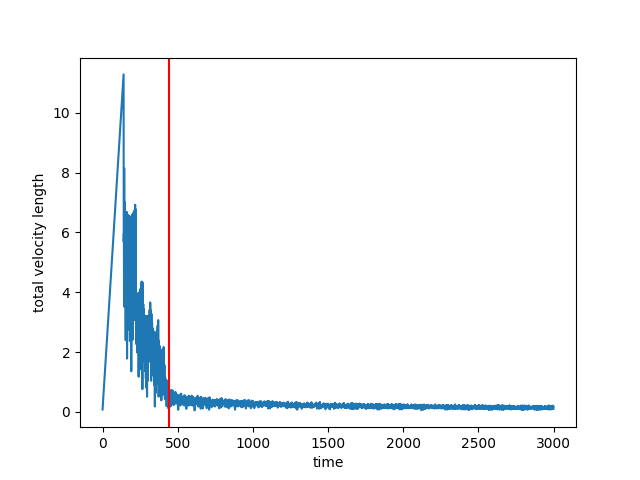
\includegraphics[scale=0.7]{images/cube_normal_3000.png}
	\caption{Szabályos, forgatás nélküli kocka ejtése közben mért mozgásvektorok összhosszúsága az idő függvényében.}
	\label{fig:cn3000}
\end{figure}
\begin{figure}[h!]
	\centering
	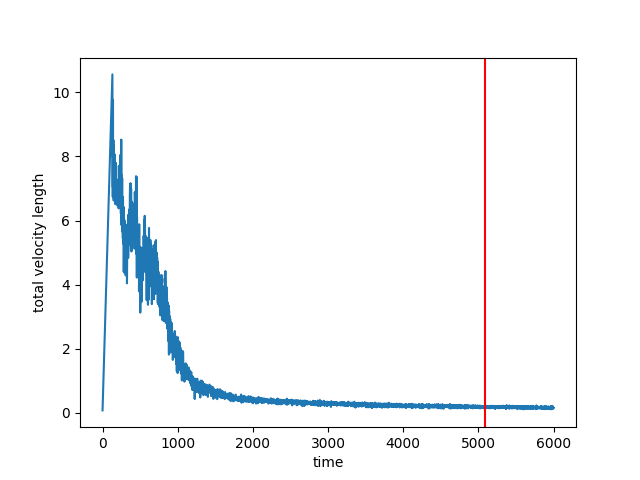
\includegraphics[scale=0.7]{images/cube_rotated_6000.png}
	\caption{Szabályos, forgatott kocka ejtése közben mért mozgásvektorok összhosszúsága az idő függvényében.}
	\label{fig:cr6000}
\end{figure}
A mért értékek alapján a mozgásvektorok összhoszzúságához tartozó küszöbérték $0.13$, a $z$ értékekre pedig $0.001$.
A \ref{fig:cn3000} és a \ref{fig:cr6000} ábrán a vörös függőleges vonal jelzi azt a pontot, amikor a program a már említett paraméterekkel megálltnak titulálta a kockát.
Látható, hogy az ideális pozícióból ejtett test sokkal hamarabb megáll, mint a forgatott.
A random elforgatott kocka nem sokkal az 5000. iteráció után megáll a talajon.
Nem szabályos test esetén arra számítunk, hogy kevesebb mint 10000 iteráció alatt meg fog állni a test.
Ha ez nem történne meg az első 10000 iterációban (egy élén vagy csúcsán pattog a végtelenségig) akkor a dobást érvénytelennek tekintjük.

\SubSection{Kiértékelés}

A módosított testeknél gyakran a dobás értéke nem rendelhető egy "felül lévő" laphoz, mint a kocka esetében, ezért célszerű a dobott értékeket a $z=0$ síkon lévő laphoz rendelni.
Hasonlóan a leállás vizsgálatához eltároljuk egy halmazban a talajon található pontok indexeit, majd megkeressük hogy melyik oldallap a részhalmaza.
\begin{python}
def faceOnGround(self):
    if not self.isStopped():
        print("not stopped")
        return -1

    onGround = set()
    for i in range(self.n):
        if self.particles[i].position[2] < ZMIN:
            onGround.add(i)

    face = []
    for i in range(len(self.faces)):
        if self.faces[i].issubset(onGround):
            face.append(i)

    if len(face) == 0:
        print("no face detected")
        return -2
    elif len(face) == 1:
        return face[0]
    else:
        print("multiple faces detected")
        return -3
\end{python}
\begin{remark}
A metódus kezeli, ha nem állt meg a test, túl kevés pont van a $z=0$ síkon, vagy ha egyszerre több oldal is a talajon van. Ezen esetekben a dobást megismételjük. 
\end{remark}
A dobássorozatokkal kapott gyakoriságokat egy tömbben tároljuk el, ahol a gyakoriságok indexei megegyeznek a hozzájuk tartozó oldallap indexével.
\begin{python}
def estimateFrequencies(self, n):
    stat = [0] * len(self.faces)

    height = 100
    dropHeight = np.array([0, 0, height], dtype=float)

    while sum(stat) < n:
        tmp = deepcopy(self)

        c = tmp.getCenter()
        tmp.translate(-1 * c)
        tmp.randRotate()
        tmp.translate(c)
        tmp.translate(dropHeight)

        i = 0
        while (not tmp.isStopped()) and i < MAXITER:
            tmp.update(TIME, GRAVITY)
            i += 1

        index = tmp.faceOnGround()
        if index >= 0:
            stat[index] += 1

    return stat
\end{python}
\Chapter{Módosító algoritmusok}

A fejezetben három heurisztikát fogunk összehasonlítani a testek optimalizálására.
Ezek közül egyet fogunk választani, amellyel \aref{ch:opt} fejezetben fogunk számolni.

A fejezetben említésre kerülő egység hossz alatt a használt koordináta rendszer egységét értjük.
A testek éleinek hossza körülbelül 50 egységnek felel meg.

\Section{Az eloszlások távolságának mérése}

Az eloszlások illetve gyakoriságok távolságát több módon is mérhetjük.
Mivel nem cél a különböző metrikákkal kapott hibaértékek összehasonlítása, ezért lényegtelen, hogy a mért és elvárt gyakoriságok és/vagy valószínűségek távolságát vizsgáljuk.
Ennek a hibának a mérésére a mért és elvárt értékek különbségéből kapható vektor normáival is megtörténhet:
\[
\vec{v} = \vec{e} - \vec{m},
\]
ahol az $\vec{e}$ az elvárt (\textit{expected}) és az $\vec{m}$ a mért (\textit{measured}) értékeket tartalmazza.

Az így kapott vektor 1-es normája által meghatározott érték megfelel a mért és elvárt adatok közötti abszolút különbségek összegével:
\[
\left\lVert\vec{v}\right\rVert_1 = \sum\limits_{i=1}^{n} |v_i|.
\]
A 2--es norma a távolságok négyzetösszegének a gyökét adja vissza:
\[
\left\lVert\vec{v}\right\rVert_2 = \sqrt{\sum\limits_{i=1}^{n} |v_i|^2}.
\]
A végtelen norma pedig a legnagyobb távolság abszolút értékét határozza meg:
\[
\left\lVert\vec{v}\right\rVert_\infty = \max\limits_{i=1}^{n} |v_i|.
\]

Lehetséges ezeken kívül az átlagos négyzetes hibának (\textit{mean squared error, MSE}) számítása, amely nem sokban tér el a 2-es norma számításától:
\[
MSE(\vec{v}) = \frac{1}{n} \sum_{i=1}^{n}(v_i)^2.
\]

Az eloszlások távolságának a mérésére a $\chi^2$-et szokták még alkalmazni, amellyel később meg lehet vizsgálni, hogy milyen szignifikancia szinten egyezik meg az elvárt és mért értéksorozat eloszlása:
\[
\chi^2=\sum_{i=1}^{n} \frac{(m_i - e_i)^2}{e_i}.
\]

A fent említett metrikák közül az MSE-t, valamint a $\chi^2$-et használják a leggyakrabban, ezért ezeket fogjuk összehasonlítani optimalizálás során.
A $\chi^2$ számítására a SciPy \cite{2020SciPy-NMeth} könyvtárban található függvényt használjuk.

\begin{table}[h!]
	\centering
	\caption{Optimalizálás során mért MSE és $\chi^2$ értékek.}
	\label{tab:compare}
	\begin{tabular}{l|c|c|}
		iteráció & MSE & $\chi^2$ \\
		\hline
		0 & 0.012605000000000002 & 309.3075 \\
		1 & 0.005730000000000002 & 133.22333333333333 \\
		2 & 0.004737500000000001 & 123.45833333333333 \\
		3 & 0.0024330000000000007 & 69.02083333333334 \\
		4 & 0.001435500000000001 & 33.730000000000004 \\
		5 & 0.0010555000000000004 & 16.908333333333335 \\
		6 & 0.00019650000000000003 & 3.2125 \\
		7 & 0.0010955000000000001 & 21.553333333333335 \\
		8 & 7.399999999999977e-05 & 1.0333333333333332 \\
		\hline
	\end{tabular}
\end{table}

Addig módosítottuk a testet, amíg a kapott MSE érték $10^{-4}$ alá nem esett, a kapott értékek \aref{tab:compare} táblázatban láthatóak.
A dobássorozatok mérete $N=1000$ volt, és a későbbi \ref{sect:facemodification} szakaszban mutatott heurisztikát használtuk.
Az értékek által meghatározott görbék alakra nagyon hasonlónak tűntek, ezért a legkisebb négyzetek módszerét alkalmazva összehasonlítjuk őket.
A számítások alapján $a_0 + a_1\cdot mse = \chi^2$, ahol $a_0 = -1.67216109, a_1 = 24742.3397$.
\begin{figure}[h!]
	\centering
	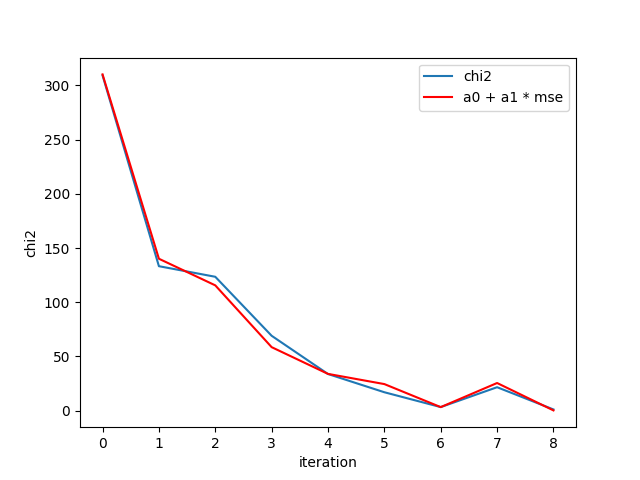
\includegraphics[scale=0.7]{images/mse_vs_chi2.png}
	\caption{A módosított MSE, és a $\chi^2$ értékek.}
	\label{fig:mse_vs_chi2}
\end{figure}
A \ref{fig:mse_vs_chi2} ábra mutatja, hogy a feltételezésünk igaz volt, a két érték konvergálása hasonló, emiatt nincs lényeges különbség a között, hogy melyiket fogjuk használni.
A végső választás azért esett a $\chi^2$-re, mert így tudjuk folyamatosan nyomon követni, hogy egy adott szignifikancia szinten el tudjuk-e fogadni a módosított test által adott gyakoriságokat.

\Section{Egyetlen pont mozgatása}
\label{sect:randmodification}

Ez a módszer a testet úgy módosítja, hogy mindig egy véletlenszerűen választott csúcspontját egy egység hosszúságú vektorral odébb helyezi.
A vektort \aref{subs:randompoint} szakaszban említett módszerrel generáljuk.
Amennyiben a módosított test dobássorozata alapján kapott gyakoriságok jobbak, mint az eredeti testé, az új testen végezzük el ugyan ezt a lépést, egyébként a módosítatlan testen.
\begin{figure}[h!]
	\centering
	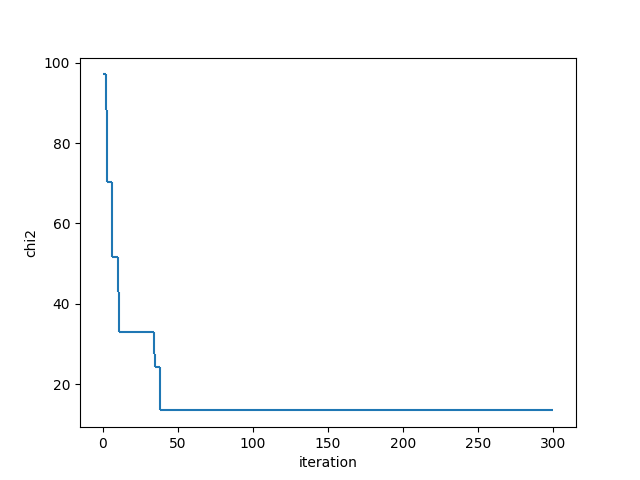
\includegraphics[scale=0.7]{images/randmodify_chi2.png}
	\caption{Egyetlen pont elmozdításával kapott test módosítása közben mért legjobb $\chi^2$ értékek.}
	\label{fig:randmodify_chi2}
\end{figure}
\Aref{fig:randmodify_chi2} grafikon egy tetraéder módosítása közben mért értékeket mutatja.
Az elvárt eloszlás $[0.1, 0.2, 0.3, 0.4]$, leállás feltételéhez az iterációk száma $300$, a dobás sorozatok mérete pedig $N=200$.
A végén kapott testtel egy $N=1000$ méretű dobássorozatnál a $\chi^2$ értéke $298.78$.
Láthatjuk hogy az így kapott érték túl nagy ahhoz hogy a testet $\alpha = 0.05$ szignifikancia szinten el tudjuk fogadni.
Ebből arra tudunk következtetni, hogy a rossz módosítást a kis méretű dobássorozaton pontatlanul mért értékek miatt helyes módosításként kezelte.
Az így elmenett hibás állapotokból gyakran nem tudja az eljárás korrigálni jó irányba a testet.

Mivel fix hosszúságú vektorral módosítjuk a testet és sosem lépünk vissza rosszabb hibaértéket adó testhez, így előfordulhat, hogy nem tudunk egy bizonyos hibaérték alá menni az optimalizálás során, mert a pontok egységsugarú környezetében található az optimális pozíciója.
Ezt úgy tudjuk kijavítani, hogy az iterációszám és a hibaértéktől függően csökkentjük a módosító vektorok hosszát.

A fent említett okok miatt érdemesebb más heurisztikával optimalizálni a testeket.

\Section{Lapméret alapján történő korrekció}
\label{sect:facemodification}

Ez az algoritmus a csúcspontokat aszerint mozgatja, hogy az oldallapokra nézve az elvárt és mért valószínűség hogyan viszonyul egymáshoz.
Ha az adott oldallap előfordulásán növelni szeretnénk, akkor a csúcsokat lap súlypontjából kifelé mutató egység hosszúságú vektorokkal mozdítjuk el, egyébként a csúcsokat a súlypont felé mozgatjuk.

\Aref{fig:facemodification} ábrán látható kék vektorok felelnek az oldallap növeléséért, a vörösek pedig annak csökkentéséért.

\begin{figure}[h!]
	\centering
	\begin{tikzpicture}
		\node [label={[shift={(-0.2,-0.1)}]$C$},inner sep=0] (C) at (4,3) {};
		\node [label={[shift={(-0.2,0)}]$P_1$},inner sep=0] (P1) at (0,0) {};
		\node [label={[shift={(0.3,-0.2)}]$P_2$},inner sep=0] (P2) at (5,7) {};
		\node [label={[shift={(0.2,0)}]$P_3$},inner sep=0](P3) at (7,2) {};
		\draw (P1) -- (P2) -- (P3) -- (P1);
		\draw [dashed] (C) -- (P1);
		\draw [dashed] (C) -- (P2);
		\draw [dashed] (C) -- (P3);
		\node [inner sep=0] (out1) at (-0.8,-0.6) {};
		\node [inner sep=0] (out2) at (5.24,7.97) {};
		\node [inner sep=0] (out3) at (7.95,1.68) {};
		\draw [->, draw=blue] (P1) -- (out1);
		\draw [->, draw=blue] (P2) -- (out2);
		\draw [->, draw=blue] (P3) -- (out3);
		\draw [dotted] (out1) -- (out2) -- (out3) -- (out1);
		\node [inner sep=0] (in1) at (0.8,0.6) {};
		\node [inner sep=0] (in2) at (4.76,6.03) {};
		\node [inner sep=0] (in3) at (6.05,2.32) {};
		\draw [->, draw=red] (P1) -- (in1);
		\draw [->, draw=red] (P2) -- (in2);
		\draw [->, draw=red] (P3) -- (in3);
		\draw [dotted] (in1) -- (in2) -- (in3) -- (in1);
	\end{tikzpicture}
	\caption{Oldallap méretének változtatása egység hosszúságú vektorral.}
	\label{fig:facemodification}
\end{figure}
\begin{figure}[h!]
	\centering
	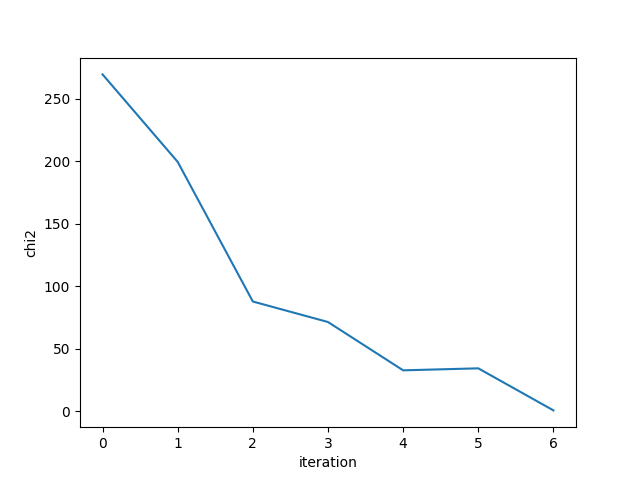
\includegraphics[scale=0.7]{images/facemodify_chi2.png}
	\caption{Az oldallapok méretének módosításával mért $\chi^2$ értékek az iterációk függvényében.}
	\label{fig:facemodify_chi2}
\end{figure}

A \ref{fig:facemodify_chi2} grafikonon látható egy tetraéder módosítása közben kapott átlagos négyzetes hibák.
A várt eloszlás $[0.1, 0.2, 0.3, 0.4]$, a dobássorozatok mérete $N=1000$, leállási feltétel pedig a $\chi^2 < 2.5$.
A végén kapott test $1000$ dobásra nézve $\chi^2 = 3.5983$ értéket adott.
Ez amiatt lehetséges, hogy a leállásnál mért értékek pontatlanság miatt közelebb voltak a várt értékekhez.
Ha kellően alacsonyra állítjuk be a küszöbértéket, akkor az ilyen hibák mellett is tudunk olyan testet kapni, amelyet egy adott $\alpha$ szignifikancia szinten el tudunk fogadni.

A \ref{subs:randompoint} szakaszban bemutatott módszerhez képest látványosan gyorsabb, és egyértelműen konvergál az elvárt eloszláshoz.
Mivel az algoritmus az aktuálisan mért eloszlásokhoz képest módosítja a lapok méretét, így az esetlegesen elkövetett hibákat folyamatosan tudja javítani, valamint mivel sokkal gyorsabban konvergál, így nyugodtan adhatunk meg nagyobb dobásméretet, amellyel tovább tudjuk csökkenteni az esetleges fals méréseket.

\Section{Módosítás az arányok figyelembe vételével}
\label{sect:ratiomodification}

Ez a folyamat szinte teljes mértékben megegyezik az előző pontban leírt metódussal.
Az egyetlen lényeges különbség annyi, hogy az oldallapokat a gyorsabb konvergencia miatt nem egység hosszú vektorokkal módosítjuk.
A módosító vektorok hossza függ az oldallapokhoz becsült és az azokhoz elvárt valószínűségek különbségétől, hogy a nagyobb eltérések esetében drasztikusabban tudjuk az oldallapokat módosítani.
Olyan eset is előfordulhat, hogy az oldallap ideális méretének eléréséhez az oldallapot fél egység hosszú vektorokkal kellene növelnünk, és ezt a méretet a \ref{sect:facemodification} szakaszban leírt függvénnyel nem tudjuk elérni.

Az algoritmus a módosító vektorok hosszát az oldallapokhoz tartozó várt és mért valószínűségek különbségével határozza meg.
Ezt a különbséget egy $\lambda$ konstanssal megszorozva tudunk a konvergencia sebességén módosítani.
Az $i$-edik oldallap $j$-edik pontját mozdító vektort az alábbi képlettel kapjuk meg:
\[
\vec{v} = (\vec{p_j} - \vec{c_i})\cdot\lambda\cdot(e_i - m_i),
\]
ahol $\vec{c_i}$ az $i$-edik oldallap középpontja, $e_i$ és $m_i$ pedig az oldalhoz tartozó elvárt, és mért gyakoriság.

\begin{figure}[h!]
	\centering
	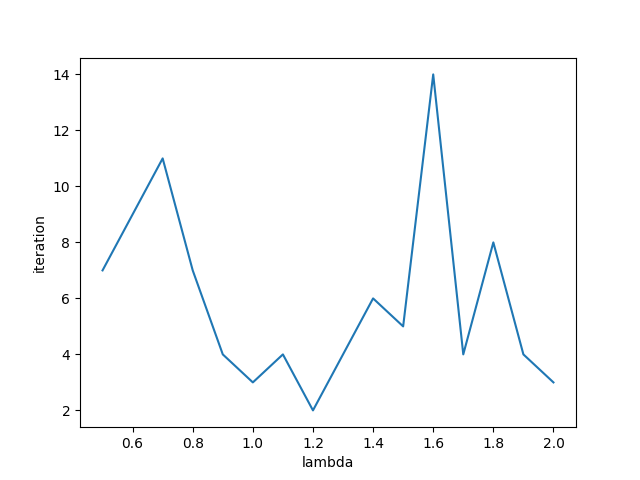
\includegraphics[scale=0.7]{images/lambdatest.png}
	\caption{Az algoritmus futásához szükséges iterációk $\lambda$ függvényében.}
	\label{fig:lambda}
\end{figure}

A \ref{fig:lambda} grafikonon láthatóak egy tetraéder módosításához szükséges iteráció számok az egyes $\lambda$ értékekhez.
Látható, hogy nem tudunk egyértelműen meghatározni ez alapján egy egyértelmű minimumot.
Hogy ezt meg tudjuk tenni minden $\lambda$ értékhez több dobássorozatot kellene elvégezni, és az így mért iterációszámokat kellene átlagolnunk.
Az egyes módosítások hossza nagyban függ a test alakjától, a várt eloszlástól, az elő mérés pontosságától, valamint a $\lambda$ értéktől.
Minden testre és azokhoz tartozó eloszlásra nézve a $\lambda$ meghatározása sokkal több időt vesz igénybe, mint ha végig egy adott konstans értékkel számolnánk.
Emiatt az optimalizálásnál $\lambda = 1$ értékkel fogunk számolni.

\begin{remark}
A tesztelések során egyik test sem került konkáv állapotba, így azt feltételezve, hogy ezzel a heurisztikával nem kapunk konvex testből konkáv testet, a konvexitás vizsgálatát a gyorsabb futási idők miatt nem végezzük el.
\end{remark}
\Chapter{Testek optimalizálása}

Érdemes megnézni, hogy egyes testeknél hogyan tudunk konvergálni különböző eloszlásokhoz.
Ehhez a \ref{sect:ratiomodification} szakaszban bemutatott heurisztikát fogjuk használni.
Addig módosítjuk a testeket, amíg az oldallapokhoz tartozó relatív hiba az általunk megadott küszöbérték alá nem esik.
Ezt a küszöböt $\chi^2$-re nézve az alábbi összefüggéssel írhatjuk fel:
\[
\chi^2 < N \cdot error^2,
\]
ahol $N$ a dobássorozat száma és $error$ az általunk megadott hibaküszöb. 

\Section{Tetraéder}

[0.1, 0.2, 0.3, 0.4]

Dark Souls Orange Dice
[1/6, 1/3, 1/3, 1/6]

\Section{Dupla tetraéder}

[1/12, 2/12, 3/12, 3/12, 2/12, 1/12]

[2/15, 2/15, 2/15, 2/15, 2/15, 1/3]

\Section{Oktaéder}

sum of 7 coin
[1/128, 7/128, 21/128, 35/128, 35/128, 21/128, 7/128, 1/128]

2 szemben lévő oldal nagyobb
[2/8, 2/8, 1/12, 1/12, 1/12, 1/12, 1/12, 1/12]

\Chapter{Összefoglalás}

A dolgozatban láthattunk néhány konkrét példát arra, hogy egy-egy diszkrét eloszláshoz hogyan tudunk becslést adni egy olyan testre, melynél a lapokhoz tartozó valószínűségek közelítik a célként kitűzött értékeket. Ehhez elkészült egy szimulációs környezet Python programozási nyelven, illetve különböző heurisztikák a test alakjának módosításához.

% A dolgozat célja, a módosító program elkészítése sikerült.
% Láthattuk, hogy képes alakzattól és eloszlástól függetlenül konvergálni az elvárt testhez.

Mivel egy olyan optimalizálási eljárásról van szó, melynél az aktuális test jósági értékének becslése statisztikai próbával ellenőrizhető, ezért a konvergencia vizsgálatánál nem várható el ezen értékek monotonitása az iterációk függvényében. Érdekes részproblémákat jelentett a dobássorozatok hosszának, és a megfelelő megbízhatósági értékek meghatározása.
A kapott eredmények értékeléséhez főként a konvergenciát szemléltető grafikonok, a konkrét hiba értékek és a statisztikai próbák eredményei szolgáltak.

A nagyobb problémákat az optimalizáló algoritmusban bevezetett $\lambda$ érték meghatározása, valamint a lassú futási idő jelentette.
Az utóbbin úgy lehetne javítani például, hogy a dobássorozatok elvégzését kiszervezzük \textit{C} programozási nyelven megírt modulba, melynek függvényei meghívhatók Python-ból.
Így tudnánk nagyobb mintára végezni a szimulációkat, pontosabb eredményeket kaphatnánk, illetve megvizsgálhatnánk a test eredeti alakja, az elvárt eloszlás és a $\lambda$ közötti összefüggést.

A tesztelések során a testeknek csak háromszög oldallapjuk volt, mivel a komplexebb esetekben az oldallapok módosításánál ügyelnünk kell arra, hogy háromnál több pont esetében a lapok csúcsai biztosan egy síkban maradjanak.
A felhasznált heurisztika a konvexitást megőrizte, de a nem háromszög oldallapokat "széttörte" több oldallapra.
További fejlesztés lehetne ehhez a problémához ennek a hibának a kezelése, vagy egy olyan módszer keresése, amely síkban tudja tartani az összes oldallapot.

A fent említett módosításokat elvégezve meg lehetne vizsgálni, hogy ugyan azt az eloszlást különböző testekből kiindulva hogyan tudja közelíteni a program (például kocka és dupla tetraéderre nézve).
Ezen felül lehetne vizsgálni, hogy a kapott test oldalainak a területe hogyan változik a módosítások közben.
Továbbá, valamilyen vizuális megjelenítőt lehetne készíteni, amivel láthatjuk a testet optimalizálás alatt, hogy hogyan változik.

A jelenlegi verzió az elvárt valószínűségeket mindig egy adott oldalhoz köti. Érdemes lenne úgy módosítani, hogy az optimalizálás közben rendelje hozzá az oldalakhoz az értékeket, és ezeknek a sorrendjét közben tudja változtatni.
Felmerülhet olyan probléma, hogy két oldalhoz tartozó elvárt értékeket folyamatosan cseréli, és emiatt egy ponton túl már nem tud jobb eredményeket adni az optimalizálási folyamat.
Ehhez egy külön leállási feltétel vizsgálatot kellene csinálni.

Az említett módosítások, bővítések nélkül is az elvárt feltételeknek megfelelően működik a program, és kellő futási idő után elég pontos eredményeket tud adni.
Az így kapott kockák elkészítése a WaveFront OBJ fájlokba történő mentése után 3D nyomtatók segítségével (természetesen a megfelelő beállítások használatával) könnyen előállíthatóak.


\clearpage

\addcontentsline{toc}{chapter}{Irodalomjegyzék}
\bibliographystyle{plain}
\bibliography{dolgozat.bib}

\newpage

\pagestyle{empty}

\noindent \textbf{\Large CD Használati útmutató}

\vskip 1cm

\noindent \textbf{A CD az alábbi jegyzékeket tartalmazza:}
\begin{itemize}
	\item\textit{dolgozat:} A szakdolgozat szövege pdf illetve LaTeX állományként.
	\item\textit{source{\_}code:} A futtatható kódok találhatóak benne.
\end{itemize}

\noindent\textbf{A \textit{source{\_}code} jegyzék tartalma:}
\begin{itemize}
	\item\textit{jelly.py:} A testek reprezentálásához szükséges osztályok találkatóak meg benne.
	\item\textit{chi2{\_}test.py:} A $\chi^2$ próba tesztelése.
	\item\textit{lambda{\_}value{\_}test.py:} A $\lambda$ érték meghatározására használt kód.
	\item\textit{mse{\_}vs{\_}chi2.py:} Az MSE és $\chi^2$ összehasonlítása legkisebb négyzetek módszerével.
	\item\textit{plane{\_}test.py:} Három pontra illeszkedő sík meghatározása.
	\item\textit{rotate{\_}test.py:} Forgatások tesztelésére szolgáló program.
	\item\textit{velocitylengthgraph.py:} A dobások során mérhető mozgásvektorok összhosszúsága által megadott grafikont kirajzoló program.
	\item\textit{tetrahedron{\_}test.py, doubletetrahedron{\_}test.py, octahedron{\_}test.py:} A tényleges optimalizáló kódok különböző testekre.
	\item\textit{graphs:} A kapott grafikonokat tartalmazó jegyzék.
	\item\textit{objects:} Az optimalizálás során elért objektumokat tartalmazza.
\end{itemize}

\noindent\textbf{A kódok futtatása:}

\textit{A programok Python $3.9.4$-ben lettek megírva.}
\textit{A futáshoz szükséges a Matplotlib, NumPy, SciPy könyvtárak telepítése.}

Az egyes kódokat parancssorból a \textit{source{\_}code} jegyzékbe való navigálás után a \textit{python} paranccsal tudjuk futtatni.


\end{document}
